\begin{figure*}[t!]
\centering
    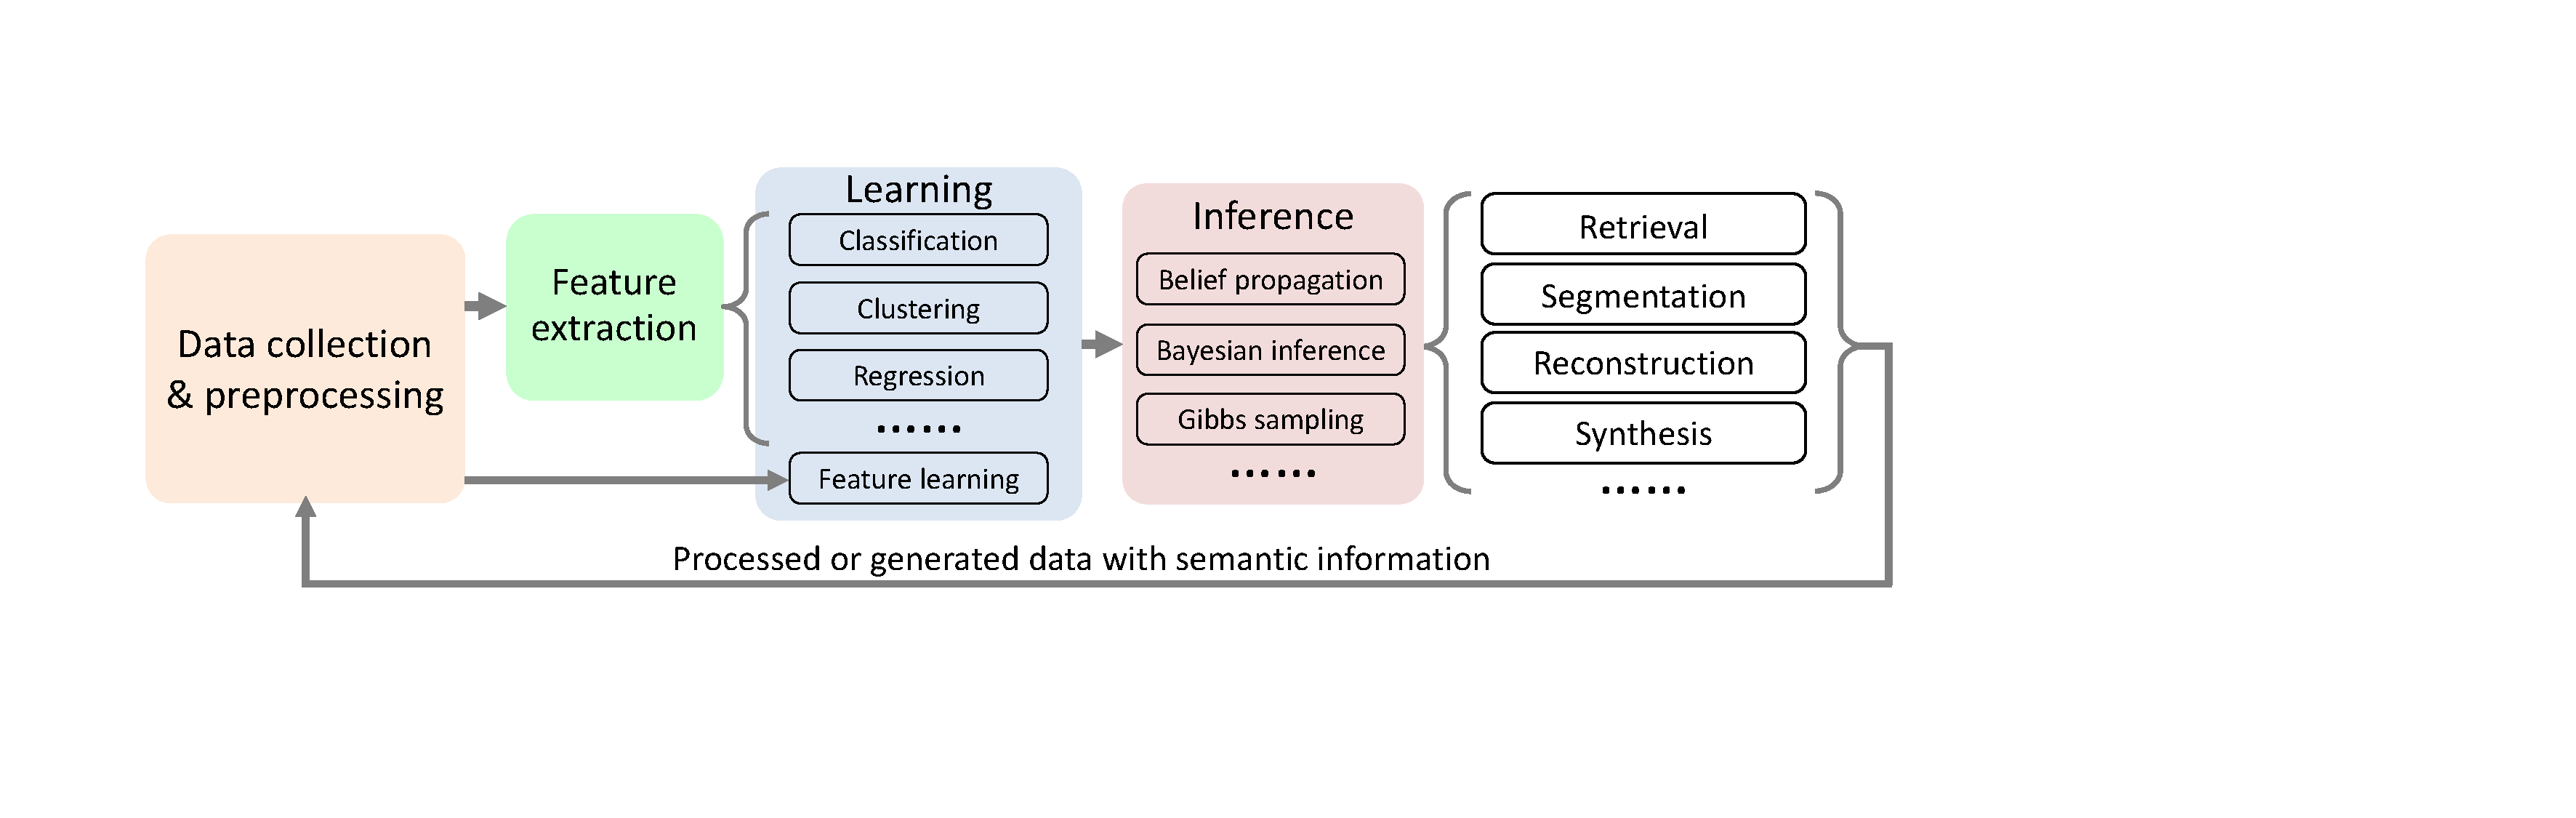
\includegraphics[width=0.9\textwidth]{fig/img/overview.pdf}
    %\vspace{-.4cm}
    \caption{
\rev{The general pipeline of data-driven geometry processing contains four major stages: data collection and preprocessing, feature extraction (or feature learning),
learning and inference. The inference supports many applications which would produce new shapes or scenes through reconstruction modeling or synthesis.
These new data, typically possessing labels for shapes or parts, can be used to enrich the input datasets and enhance the learning tasks in future, forming a data-driven geometry processing loop.}}
    \label{fig:overview}
\end{figure*}

